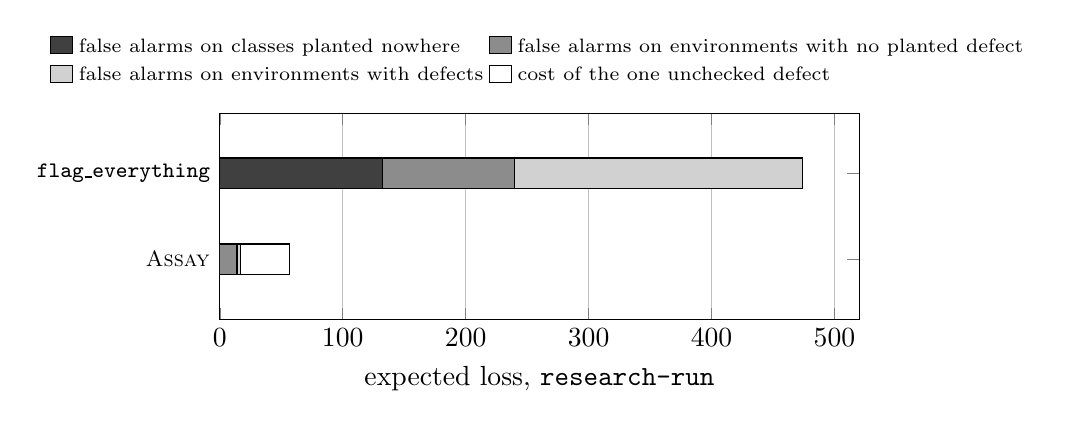
\begin{tikzpicture}
\begin{axis}[xbar stacked, width=0.8\linewidth, height=4.2cm, xmin=0, xmax=520,
  ytick={0,1}, ymin=-0.7, ymax=1.7,
  yticklabels={\textsc{Assay},\texttt{flag\_everything}}, yticklabel style={font=\footnotesize},
  xlabel={expected loss, \texttt{research-run}}, bar width=11pt, xmajorgrids,
  legend style={at={(0.5,1.08)}, anchor=south, font=\scriptsize, legend columns=2, draw=none},
  legend cell align=left]
\addplot[fill=black!75] coordinates {(132,1) (0,0)};
\addplot[fill=black!45] coordinates {(108,1) (14,0)};
\addplot[fill=black!18] coordinates {(234,1) (3,0)};
\addplot[fill=white, draw=black] coordinates {(0,1) (40,0)};
\legend{false alarms on classes planted nowhere, false alarms on environments with no planted defect, false alarms on environments with defects, cost of the one unchecked defect}
\end{axis}
\end{tikzpicture}
